\subsection{Hyperbolic Paraboloids}
\noindent
Hyperbolic paraboloids have the form
\begin{equation*}
	z = x^2 - y^2.
\end{equation*} 
They are not radially symmetric and look like a saddle or Pringle's chip.

\begin{figure}[H]
	\centering
	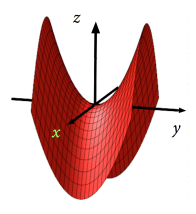
\includegraphics[width=0.33\textwidth]{./Images/differentialMultivariableCalculus/hyperbolic_paraboloid.png}
	\caption{A hyperbolic paraboloid}
\end{figure}